\chapter{Specification of needs}
\section*{Introduction}
In this chapter, we will identify the actors, then we will specify the functional and non-functional needs that the proposed solution must meet. Finally, we present the use case diagrams explaining our application's main functionalities.
\section{Identification of actors}
An actor represents an external entity that interacts directly with the
system. It can be either a human person or a system. We distinguish
two types of actors, the main actor, and a secondary actor. Indeed,
a principal actor obtains an observable result of the system while a
secondary actor is asked for additional information.\\
\subsection*{Main actors}
\textbf{Community Manager}\\
The community manager is the first main user of our application who should be able to :
\begin{itemize}
\item[•] Choose the community that he has the right to access and manage.
\item[•] Consult users of a specific community inside a well-organized table with pagination options.
\item[•] Filter said users by name, user-name, Salesforce account name, status( active or not active ), and Salesforce profile.
\item[•] Consult and update the details of each user.
\item[•] Activate users within a specific community.
\item[•] Deactivate users within a specific community.
\item[•] Send a "Welcome to community" email to a specific active user.
\item[•] Send a "Reset password" email to a specific active user.
\item[•] Add one or multiple users at once to a specific community.
\end{itemize}
In case when the community manager has a Salesforce role he will be also able to :
\begin{itemize}
\item[•] Add one or multiple users at once to a specific community.
\end{itemize}
\textbf{Salesforce Administrator}\\
The Salesforce administrator is the second main user of our application who should be able to :
\begin{itemize}
\item[•] Perform all the actions, mentioned above, that the community manager can.
\item[•] Consult a bar chart that shows the number of logins of each user within the selected community.
\item[•] Filter chart results by the period between two specific dates.
\item[•] Consult details about each user displayed in the chart.
\item[•] Update the Salesforce user license for each user displayed in the chart.
\item[•] Consult users failed login attempts to a specific community inside a well-organized table with pagination options.
\item[•] Filter said login attempts by name, user-name, status( Invalid password, No community access, etc... ) and event date and time.
\item[•] Consult detailed information about each login attempt.
\item[•] Send a security warning email to the account owner about the login attempt event.
\item[•] Access a Chatbot that provides information about the selected community or the Salesforce organization.


\end{itemize}
\subsection*{Secondary actors}
\textbf{Salesforce System}\\
This actor is the system, previously developed and deployed in a cloud server by the Salesforce organization, interactable through our application, and it's responsible for :
\begin{itemize}
\item[•] Sending an automatic "Welcome to community" email upon adding a new member to the community by our application user.  
\item[•] Sending an automatic "Welcome to community" email upon activating a previously deactivated user by our application user.
\item[•] Generating reset password URL upon sending a "Reset password" email to a community member by our application user.
\item[•] Tracking users' successful and failed login attempts and saving them to the organization database.

\end{itemize}
\section{Functional Needs}
Functional needs are expressed by the user of the application
which makes it possible to identify the functionalities of this application.\\
In our
case, the functional needs are:
\begin{itemize}
\item Choice of the community:\\
Select the community to which we will manage the users.

\item Manage users:\\
The system must allow users to be managed with the functionalities of activation,
deactivation, modification, and consultation of the list of users via a data table.
Creation of different filters that allow us to facilitate the navigation of the list of users.

\item Manage connection history:\\
Create a chart that shows the number of user connections per day, week, year, or
according to a well-determined date. This allows the administrator to modify the user’s license.


\item Offer a synthetic dashboard:\\
Allowing the system administrator / the community manager to visualize the KPIs (Key Performance Indicators) of his organization / community.


\end{itemize}
\section{Non-functional Needs}
Non-functional requirements represent the characteristics of the system.
They relate to the constraints to be taken into consideration to set up
an adequate solution.\\
For our application, the non-functional requirements are:
\begin{itemize}
\item Security:\\
Access to information is only possible after verification of privileges and access rights,
for example Authentication, Redirections.

\item Ergonomics and user-friendliness:\\
The application will provide a user-friendly and easy-to-use interface that does not
require any prerequisites, so it can be used by all types of users (even non-computer specialists).

\item Extensibility and maintainability:\\
The architecture of the application will allow the evolution and maintenance (addition
or deletion or update) at the level of its various modules in a flexible manner.

\item Performance:\\
The application must be efficient, i.e. the system must react within a period that does
not exceed 5 seconds, whatever the action of the application.

\item Availability:\\
The application will be available on 24/24, and 7/7 except during the maintenance period.

\end{itemize}
\section{Use case diagrams}
In this section, we will highlight the system's functionalities to be
from the functional needs mentioned above based on the UML(Unified Modeling Language) diagrams which group together all the use cases of the system.
\subsection{Global use case diagram}
The following figure illustrates the global use case diagram of our application
\begin{figure}[H]%
    \center   
    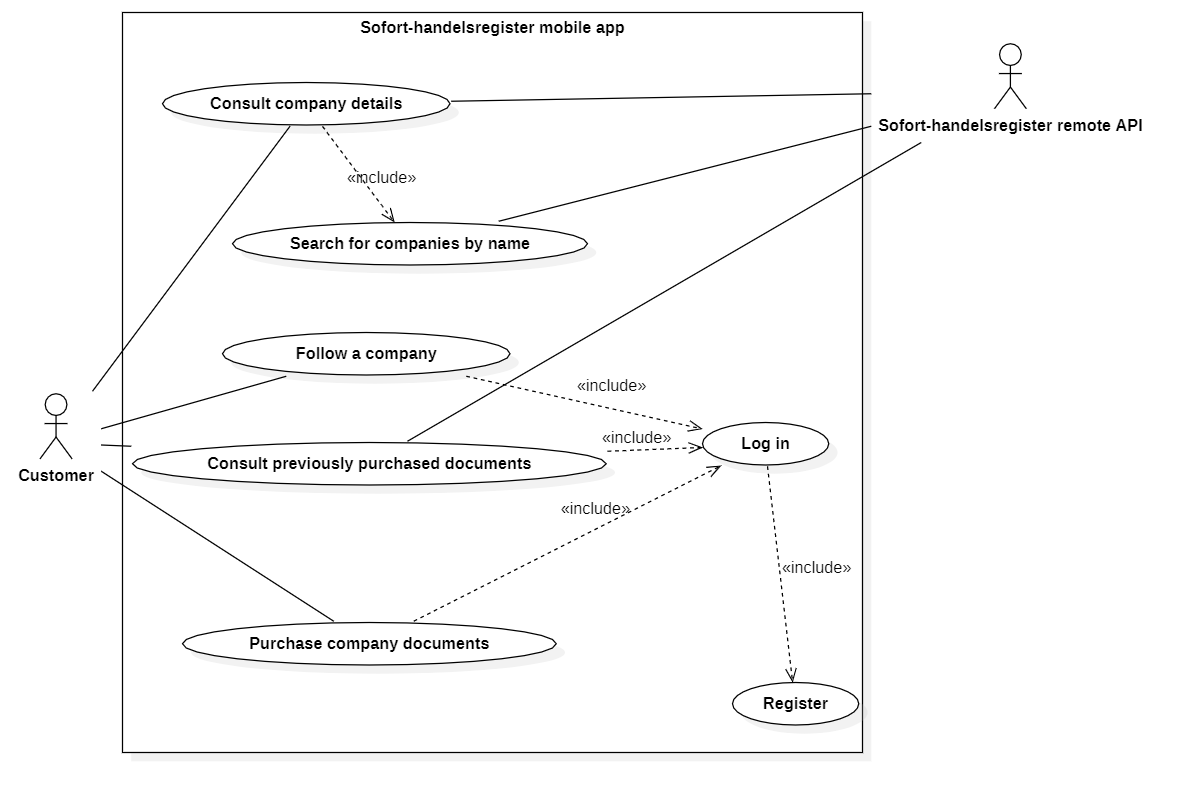
\includegraphics[scale=0.45]{UC_global.png}
    \caption{Global use case diagram}
\end{figure}
\subsection{Use case refinement}
In this section, we will detail the main use cases.
\subsubsection{Register use case refinement}
In our application, a customer must register before benefiting from the service of purchasing a document through our application.\\
The following figure shows the Register use case diagram.
\begin{figure}[H]%
    \center   
    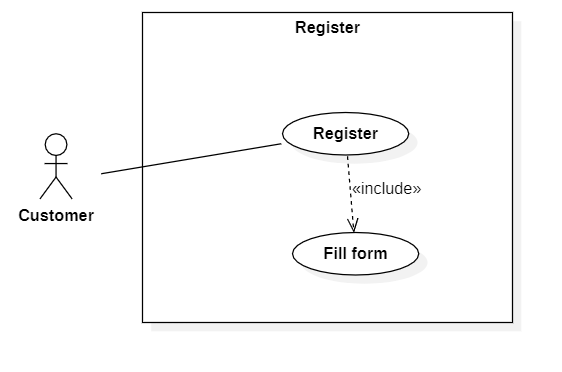
\includegraphics[scale=0.5]{UC_r.png}
    \caption{Register use case diagram}
\end{figure}
\pagebreak
The following table details the tasks to be performed by the customer to register
to our app.

\begin{table}[H]
\begin{tabular}{|ll|}
\hline
\multicolumn{2}{|c|}{\textbf{Summary}}                                                                                                                                                                                                                                                                                                                                                                             \\ \hline
\multicolumn{1}{|l|}{Title}                         & Register                                                                                                                                                                                                                                                                                                                                                     \\ \hline
\multicolumn{1}{|l|}{Objectif}                      & \begin{tabular}[c]{@{}l@{}}Allowing the user to register to be able to purchase documents\\  and follow companies through the application\end{tabular}                                                                                                                                                                                                       \\ \hline
\multicolumn{1}{|l|}{Actors}                        & Customer                                                                                                                                                                                                                                                                                                                                                     \\ \hline
\multicolumn{2}{|c|}{\textbf{Description of sequences}}                                                                                                                                                                                                                                                                                                                                                            \\ \hline
\multicolumn{1}{|l|}{Pre-condition}                 & \begin{tabular}[c]{@{}l@{}}User should start the application and go to the registration\\ interface.\end{tabular}                                                                                                                                                                                                                                            \\ \hline
\multicolumn{1}{|l|}{Post-condition}                & \begin{tabular}[c]{@{}l@{}}The user is registered and his contact details are saved in\\ the database.\end{tabular}                                                                                                                                                                                                                                          \\ \hline
\multicolumn{1}{|l|}{\textbf{Normal scenario}}      & \begin{tabular}[c]{@{}l@{}}1. The user accesses the registration interface. \\ 2. The user completes the form and complies. \\ 3. Registration is completed.\end{tabular}                                                                                                                                                                       \\ \hline
\multicolumn{1}{|l|}{\textbf{Alternative scenario}} & \begin{tabular}[c]{@{}l@{}}1. Empty fields: The system sends an error message:\\ You must complete all fields \\ 2. The email or password entered is not valid:\\ The system displays an error message describing \\ the validation conditions for these fields. \\ 3. The email is already in use: An alert is sent by the system\end{tabular} \\ \hline
\multicolumn{1}{|l|}{\textbf{Non functional constraints}}    & \begin{tabular}[c]{@{}l@{}}1. The interface must be ergonomic. \\ 2. Error messages should be understandable and clear.\end{tabular}                                                                                                                                                                                                                         \\ \hline
\end{tabular}
\caption{Register use case}

\end{table}
\pagebreak
\subsubsection{Login use case refinement}
In our application, a customer must log in before benefiting from the service of purchasing a document through our application and tracking a specific company through notifications.\\
The following figure shows the Login use case diagram.
\begin{figure}[H]%
    \center   
    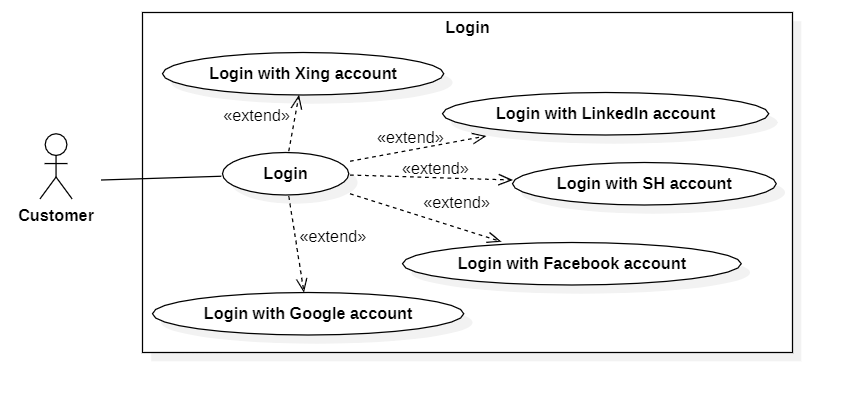
\includegraphics[scale=0.5]{UC_l.png}
    \caption{Login use case diagram}
\end{figure}
\pagebreak
The following table details the tasks to be performed by the customer to log in
to our app.
\begin{table}[H]
\begin{tabular}{|ll|}
\hline
\multicolumn{2}{|c|}{\textbf{Summary}}                                                                                                                                                                                                                                                                                                                               \\ \hline
\multicolumn{1}{|l|}{Title}                               & Login                                                                                                                                                                                                                                                                                                    \\ \hline
\multicolumn{1}{|l|}{Objectif}                            & \begin{tabular}[c]{@{}l@{}}Allowing the user to login to be able to purchase documents\\  and follow companies through the application\end{tabular}                                                                                                                                                      \\ \hline
\multicolumn{1}{|l|}{Actors}                              & Customer                                                                                                                                                                                                                                                                                                 \\ \hline
\multicolumn{2}{|c|}{\textbf{Description of sequences}}                                                                                                                                                                                                                                                                                                              \\ \hline
\multicolumn{1}{|l|}{Pre-condition}                       & \begin{tabular}[c]{@{}l@{}}User should start the application and go to the log in \\ interface.\end{tabular}                                                                                                                                                                                             \\ \hline
\multicolumn{1}{|l|}{Post-condition}                      & \begin{tabular}[c]{@{}l@{}}The user is logged in and his session is cached in\\ the application.\end{tabular}                                                                                                                                                                                            \\ \hline
\multicolumn{1}{|l|}{\textbf{Normal scenario}}            & \begin{tabular}[c]{@{}l@{}}1. The user accesses the login interface. \\ 2. The user completes the form and complies or \\ he clicks on one of the social media buttons\\ and completes the external login process. \\ 3. Login is completed.\\ 4. The login token is cached within the application.\end{tabular} \\ \hline
\multicolumn{1}{|l|}{\textbf{Alternative scenario}}       & \begin{tabular}[c]{@{}l@{}}1. Empty fields: The system sends an error message:\\ You must complete all fields \\ 2. The email or password entered is not valid:\\ The system displays an error message describing \\ the validation conditions for these fields.\end{tabular}                \\ \hline
\multicolumn{1}{|l|}{\textbf{Non functional constraints}} & \begin{tabular}[c]{@{}l@{}}1. The interface must be ergonomic. \\ 2. Error messages should be understandable and clear.\end{tabular}                                                                                                                                                                     \\ \hline
\end{tabular}
\caption{Login use case}
\end{table}
\pagebreak
\subsubsection{Company search use case refinement}
The following figure illustrates the use case diagram "Company Search"
\begin{figure}[H]%
    \center   
    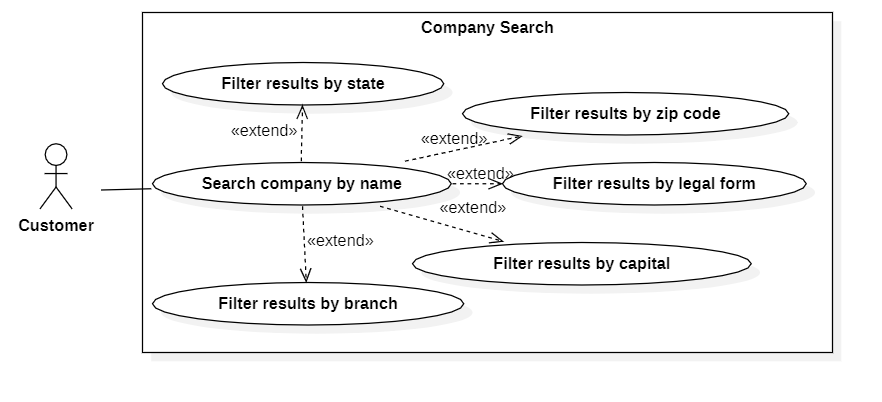
\includegraphics[scale=0.5]{UC_s.png}
    \caption{Company Search use case diagram}
\end{figure}
\pagebreak
The following table details the tasks to be performed by the customer to search for companies within our app.
\begin{table}[H]
\begin{tabular}{|ll|}
\hline
\multicolumn{2}{|c|}{\textbf{Summary}}                                                                                                                                                                                                                                                                                                                                                                                                                                     \\ \hline
\multicolumn{1}{|l|}{Title}                               & Company Search                                                                                                                                                                                                                                                                                                                                                                                                 \\ \hline
\multicolumn{1}{|l|}{Objectif}                            & \begin{tabular}[c]{@{}l@{}}Allowing the user to search for specific \\ companies through the application\end{tabular}                                                                                                                                                                                                                                                                                          \\ \hline
\multicolumn{1}{|l|}{Actors}                              & Customer                                                                                                                                                                                                                                                                                                                                                                                                       \\ \hline
\multicolumn{2}{|c|}{\textbf{Description of sequences}}                                                                                                                                                                                                                                                                                                                                                                                                                    \\ \hline
\multicolumn{1}{|l|}{Pre-condition}                       & \begin{tabular}[c]{@{}l@{}}User should start the application and go to the \\ search company interface.\end{tabular}                                                                                                                                                                                                                                                                                           \\ \hline
\multicolumn{1}{|l|}{Post-condition}                      & \begin{tabular}[c]{@{}l@{}}The user chooses a company from the list of results \\ and consults details about it.\end{tabular}                                                                                                                                                                                                                                                                                  \\ \hline
\multicolumn{1}{|l|}{\textbf{Normal scenario}}            & \begin{tabular}[c]{@{}l@{}}1. The user accesses the company search interface. \\ 2. The user types the company name \\ or the first letters of it. \\ 3. The user may choose \\ a specific state, a legal form, or \\  a branch to filter the results.\\ 4. The user may also type zip code \\ or capital as a filter. \\ 5. The user consults details about companies\\ from the list of results.\end{tabular} \\ \hline
\multicolumn{1}{|l|}{\textbf{Alternative scenario}}       & \begin{tabular}[c]{@{}l@{}}1. No results: The system sends a message:\\ No results were found with the given parameters \\ 2. No internet: The system sends an error message:\\ No internet connection found.\end{tabular}                                                                                                                                                                                     \\ \hline
\multicolumn{1}{|l|}{\textbf{Non functional constraints}} & \begin{tabular}[c]{@{}l@{}}1. The interface must be ergonomic. \\ 2. Error messages should be understandable and clear.\end{tabular}                                                                                                                                                                                                                                                                           \\ \hline
\end{tabular}
\caption{Company Search}
\end{table}
\pagebreak
\subsubsection{Follow Company use case refinement}
The following figure illustrates the use case diagram "Follow Company"
\begin{figure}[H]%
    \center   
    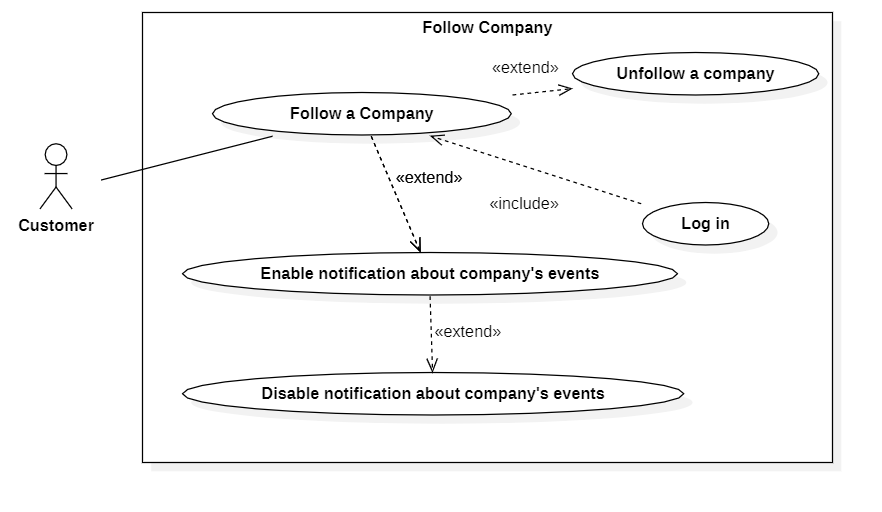
\includegraphics[scale=0.5]{UC_f.png}
    \caption{Follow Company use case diagram}
\end{figure}
\pagebreak
The following table details the tasks to be performed by the customer to follow a company within our app.
\begin{table}[H]
\begin{tabular}{|ll|}
\hline
\multicolumn{2}{|c|}{\textbf{Summary}}                                                                                                                                                                                                                                                                                                                                                                                                                                                                  \\ \hline
\multicolumn{1}{|l|}{Title}                               & Follow Company                                                                                                                                                                                                                                                                                                                                                                                                                              \\ \hline
\multicolumn{1}{|l|}{Objectif}                            & \begin{tabular}[c]{@{}l@{}}Allowing the user to follow specific \\ companies to receive notifications\\ about its events through the application\end{tabular}                                                                                                                                                                                                                                                                               \\ \hline
\multicolumn{1}{|l|}{Actors}                              & Customer                                                                                                                                                                                                                                                                                                                                                                                                                                    \\ \hline
\multicolumn{2}{|c|}{\textbf{Description of sequences}}                                                                                                                                                                                                                                                                                                                                                                                                                                                 \\ \hline
\multicolumn{1}{|l|}{Pre-condition}                       & \begin{tabular}[c]{@{}l@{}}User should start the application, be logged in, \\ search for a specific company and \\ access the consult company details interface.\end{tabular}                                                                                                                                                                                                                                             \\ \hline
\multicolumn{1}{|l|}{Post-condition}                      & The tracked company is added to the user's follow list.                                                                                                                                                                                                                                                                                                                                                                                     \\ \hline
\multicolumn{1}{|l|}{\textbf{Normal scenario}}            & \begin{tabular}[c]{@{}l@{}}1. The user accesses the consult company interface. \\ 2. The user taps the follow button. \\ 3. The user may choose \\ to unfollow the company or enable event notifications.\\ \\ 4. Upon activating notifications, \\ the user will receive notifications through the application\\ when a notice is published about said company. \\ 5. The user can tap the notification to access the notice.\end{tabular} \\ \hline
\multicolumn{1}{|l|}{\textbf{Alternative scenario}}       & \begin{tabular}[c]{@{}l@{}}1. Not logged in: The system sends an error message:\\ You must be logged in to follow a company.\end{tabular}                                                                                                                                                                                                                                                                                                   \\ \hline
\multicolumn{1}{|l|}{\textbf{Non functional constraints}} & 1. The notification must be as close to real-time as possible                                                                                                                                                                                                                                                                                                                                                                                  \\ \hline
\end{tabular}
\caption{Follow Company use case}
\end{table}
\pagebreak
\subsubsection{Purchase Documents use case refinement}
The following figure illustrates the use case diagram "Purchase Documents"
\begin{figure}[H]%
    \center   
    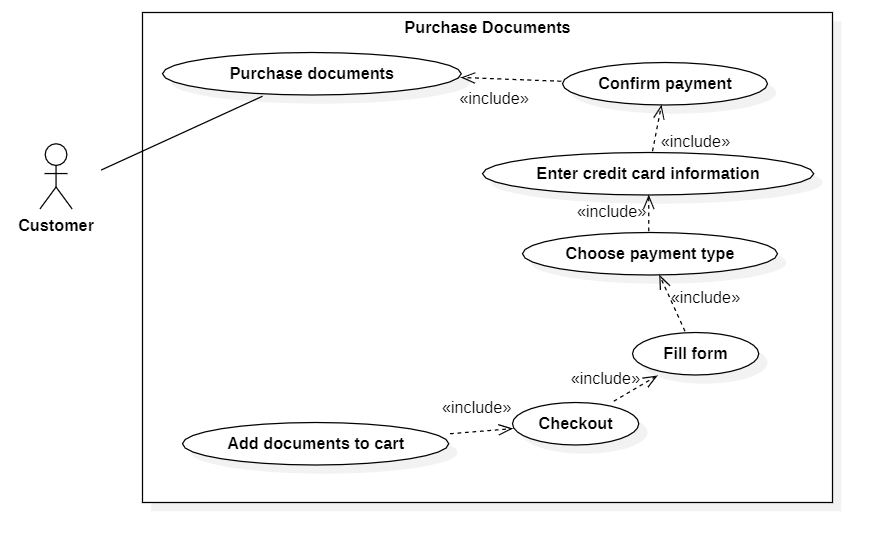
\includegraphics[scale=0.5]{UC_p.png}
    \caption{Purchase Documents use case diagram}
\end{figure}
\pagebreak
The following table details the tasks to be performed by the customer to purchase documents within our app.

\begin{table}[H]
\begin{tabular}{|ll|}
\hline
\multicolumn{2}{|c|}{\textbf{Summary}}                                                                                                                                                                                                                                                                                                                                                                                                                                                                                                 \\ \hline
\multicolumn{1}{|l|}{Title}                               & Purchase Documents                                                                                                                                                                                                                                                                                                                                                                                                                                                         \\ \hline
\multicolumn{1}{|l|}{Objectif}                            & \begin{tabular}[c]{@{}l@{}}Allowing the user to purchase official documents \\ about the consulted company, if they are available.\end{tabular}                                                                                                                                                                                                                                                                                                                            \\ \hline
\multicolumn{1}{|l|}{Actors}                              & Customer                                                                                                                                                                                                                                                                                                                                                                                                                                                                   \\ \hline
\multicolumn{2}{|c|}{\textbf{Description of sequences}}                                                                                                                                                                                                                                                                                                                                                                                                                                                                                \\ \hline
\multicolumn{1}{|l|}{Pre-condition}                       & \begin{tabular}[c]{@{}l@{}}User should start the application, be logged in, \\ search for a specific company, \\ access the consult company details interface \\ and scroll to the documents section.\end{tabular}                                                     \\ \hline
\multicolumn{1}{|l|}{Post-condition}                      & \begin{tabular}[c]{@{}l@{}}The purchased documents are added to their user's purchased documents\\ interface where he can download them on demand.\end{tabular}                                                                                                                                                                                                                                                                                                            \\ \hline
\multicolumn{1}{|l|}{\textbf{Normal scenario}}            & \begin{tabular}[c]{@{}l@{}}1. The user accesses the consult company interface. \\ 2. The user taps the wanted documents. \\ 3. The documents will be added to the shopping cart \\ 4. Upon checkout, the user will be redirected to the payment interface\\ 5. The user fills in the contact information form\\ 6. The user chooses the payment method\\ 7. The user enters credit card details\\ 8. The user confirms the payment\\ 9. Purchase is completed\end{tabular} \\ \hline
\multicolumn{1}{|l|}{\textbf{Alternative scenario}}       & \begin{tabular}[c]{@{}l@{}}1. Not logged in: The system sends an error message:\\ You must be logged in to purchase documents.\end{tabular}                                                                                                                                                                                                                                                                                                                                \\ \hline
\multicolumn{1}{|l|}{\textbf{Non functional constraints}} & \begin{tabular}[c]{@{}l@{}}1. The interface must be ergonomic. \\ 2. Error messages should be understandable and clear.\\ 3. The payment must be as secure as possible\end{tabular}                                                                                                                                                                                                                                                                                        \\ \hline
\end{tabular}
\caption{Purchase Documents use case}
\end{table}
\pagebreak
\section*{Conclusion}
In this chapter, we have described the specification phases of the
needs of our developed application to identify the different actors
as well as the features and services that our application must provide.\\
We have detailed these features with use case diagrams. The next chapter will be devoted to the design phase.